\section{Exécution \& tests} % (fold)
\label{sec:execution}

Pour ce projet, nous avons effectué des tests de validation sur quelques fonctions, afin de s'assurer que celles-ci marchaient correctement, et pouvoir plus facilement isoler les problèmes. 
De même, le code a été segmenté pour permettre une lecture plus aisée de l'ordre dans lequel s'effectuent les diverses opérations.

\section{Performances} % (fold)
\label{sec:perf}

Les courbes de performances ont été tracées avec gnuplot sur la version \og jouet \fg. Nous pouvions donc\\

Dans un premier temps, nous avons comparé la distribution linéaire et la distribution des restes chinois, sans le vol de taches. Alors que la distribution linéaire n'est pas très efficace, la distribution des restes chinois permet de mieux répartir les taches couteuses entre les processus, ces taches couteuses étant contiguës dans le tableau d'attribution des tests (cela se retrouve dans le calcul des rayons, où les taches avec un temps de calcul élevé sont dans la même régions).

Dans un second temps, nous avons observé les performances de la distribution linéaire avec le vol de taches.

%\begin{figure}[H]
%\centering
%\includegraphics[width=0.8\textwidth]{diff.png}
%\caption{Temps d'exécution des différentes parties du programme}
%\label{fig:diff}
%\end{figure}

Sur la figure \ref{fig:sp}, on peut voir qu'avec le vol de tâche, on peut être beaucoup plus rapide qu'en attribuant les tâches de manière statique aux différents processus. En effet, pour la version multithreadé, nous ne faisions qu'attribuer des tâches d'une longueur définie à un certain processus, et celui-ci les parallélisait ensuite parmi ses threads. Ainsi, les processus ayant les tâches les plus longues, pourtant bien moins nombreuses. Sur cet exemple, nous affections 10 tâches de longueur 5e+6 $\mu s$ au Processeur 1.
\begin{figure}[H]
\centering
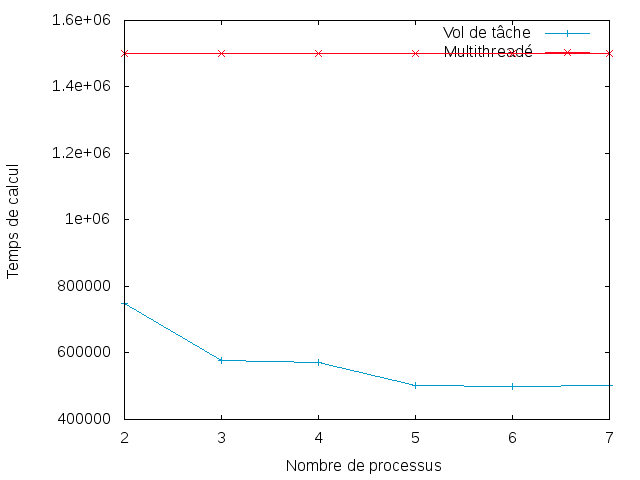
\includegraphics[width=0.8\textwidth]{stats.png}
\caption{Le vol de tâche permet d'être plus rapide}
\label{fig:sp}
\end{figure}

% section \ (end)
